\documentclass[10pt,twocolumn]{article}
\usepackage[a4paper,margin=1.8cm]{geometry}
\usepackage{amsmath,amssymb,booktabs,graphicx,microtype}
\usepackage[numbers,sort&compress]{natbib}
\usepackage[colorlinks=true,allcolors=blue]{hyperref}
\setlength{\columnsep}{0.65cm}
\title{Calibration Objectives and Computation in Strong-Teacher GNN-to-SNN Conversion}
\author{Anonymous authors}
\date{14 November 2026}
\begin{document}
\maketitle
\begin{abstract}
Frozen graph classifiers expose a practical question for low-timestep conversion: does matching final graph logits improve calibration beyond reconstructing local activations? We compare six conditions using the same pretrained residual GCNs, training examples and update budget on MNIST and CIFAR10 superpixel classification. Matched membrane conditions calibrate 693 initial-membrane values while retaining hard signed eight-level events. Across three teacher seeds per task, frozen test differences between graph-logit and local reconstruction objectives range from $-0.18$ to $+0.20$ percentage points at one or two active ticks; validation and test results differ in direction. These official splits have historical project exposure, so the endpoints are descriptive. Output error correlates with prediction flips more closely than node error, while ideal-site interventions locate a substantial short-prefix deficit upstream: restoring the first node nonlinearity alone closes about 54\% and 24\% of the one-tick teacher-disagreement gaps. Graph-level objective choice consequently requires evidence beyond error correlation. Synchronized RTX 3060 measurements show that the current diagnostic conversion core takes about 2.4--3.1 times the teacher's time at one tick. The study separates fidelity, calibration effectiveness and software execution cost, with small objective-dependent gains and no general method advantage established in the tested regime.

\end{abstract}

\section{Introduction}
Graph classification introduces two distinct targets for ANN-to-SNN calibration: reconstructing node activations and preserving the final graph prediction. Message propagation and pooling can amplify or cancel node errors, so their average magnitude alone need not determine the prediction error. This observation motivates task-level calibration, but leaves an empirical question: does a graph-output objective improve conversion beyond a local reconstruction objective when both receive the same frozen teacher, examples, parameters and update budget?

We study this question on MNIST and CIFAR10 superpixel graph classification using four-layer residual GCN teachers adapted from the Benchmarking GNNs architecture~\citep{dwivedi2023}. The teacher test accuracies average 91.02\% and 54.94\%, respectively, across three training seeds. A differential conversion adapted from fixed public source units closely matches the teacher at four or eight active ticks, while one tick leaves appreciable classification loss. These settings distinguish a substantial short-prefix problem from the small residual errors at longer prefixes.

Our comparison changes only the calibration objective for 693 channelwise initial-membrane values. It includes local activation reconstruction, graph-logit reconstruction, their fixed mixture, an output-bias control, and a target-correspondence counterfactual. We retain the original calibration failure and a single smaller-step correction, then freeze the configuration for three-teacher evaluation. Per-graph records separate accuracy, teacher agreement, reconstruction error and decision margin. Independent measurements distinguish scalar event counts, dense arithmetic and synchronized GPU time.

The resulting evidence addresses the practical value and limits of objective choice. A basic readout error identity provides motivation; its usefulness as a calibration principle depends on the matched experiments. The contribution is an empirical characterization of this conversion regime, with the supported conclusions stated in Section~\ref{sec:results}.

\section{Related Work}
Post-conversion calibration already uses ANN knowledge to correct activation mismatch. Li et al.~\citep{li2021} study layerwise reconstruction and adjust parameters including biases and initial potentials. Distribution-based threshold and potential initialization~\citep{bojkovic2024} further establishes potential calibration as an existing technique. Temporal misalignment is another recognized source of low-timestep conversion error~\citep{bojkovic2025}. These precedents motivate a strong local reconstruction control and a restricted interpretation of a learned initial state.

Differential coding transmits changes in represented activations and decodes them with time-dependent weights~\citep{huang2025}. We use the public eight-level signed MTH differential unit in a project adaptation for residual graph convolutions. Its threshold histogram and graph placement differ from the original complete conversion procedure. One-Spike conversion already includes GCNs~\citep{onespike2024}, so converting a graph operator alone does not establish novelty. Coarse-to-fine calibration for language models~\citep{fas2025} also makes output-aware calibration a relevant cross-domain precedent. The question here is the controlled effect of objective choice in strong-teacher, whole-graph classification.

\section{Conversion and Calibration}
\subsection{Teacher and event semantics}
For fixed normalized graph propagation $A$, the residual teacher layers are
\begin{equation}
 H_{\ell+1}=H_\ell+\operatorname{ReLU}(A H_\ell W_\ell+b_\ell).
\end{equation}
An embedding produces $H_0$ from node features and positions. Mean pooling followed by a three-linear-layer MLP produces ten graph logits. Evaluation-time batch normalization is folded into the graph convolution. Four convolutional branches and the two hidden MLP ReLUs form the six converted sites.

Each site emits either zero or one signed scalar event with magnitude $\theta_j 2^{-k}$, $k\in\{0,\ldots,7\}$. Threshold comparisons use the public unit's $0.75$ margin; negative emission additionally requires sufficient cumulative output. These are graded signed events. With zero-latched baseline current, define site current $c_t$, membrane $v_t$, cumulative quantity $C_t$, and represented input/output $a_t,b_t$. Before event selection,
\begin{align}
 \widetilde v_t&=v_{t-1}+c_t+a_{t-1}-b_{t-1},\\
 \widetilde C_t&=C_{t-1}+b_{t-1}.
\end{align}
After selecting $s_t$ from the signed threshold ladder,
\begin{align}
 v_t&=\widetilde v_t-s_t,& C_t&=\widetilde C_t+s_t,\\
 a_t&=a_{t-1}+c_t/t,& b_t&=b_{t-1}+s_t/t.
\end{align}
The decoded activation is $\widehat H(T)=\sum_{t=1}^T s_t/t$. The static input and affine biases enter at the first active tick. The classifier uses the same weighted event sum. $T$ counts active ticks; a non-emitting zero-latch call is separate.

\subsection{Why local and graph errors can differ}
Consider a fixed linear propagation $A$, weight matrix $W$ and linear graph readout $R$. If $E=\widehat H-H$, equal bias conventions give
\begin{equation}\label{eq:linear}
 \Delta Y=RA(EW).
\end{equation}
Equal Frobenius norms of $E$ can therefore yield unequal graph errors through directional sensitivity and cancellation. Equation~\eqref{eq:linear} applies to this fixed linear segment. The residual ReLUs and nonlinear classifier require separate treatment, while dynamic gated graph propagation changes the operator itself. Accordingly, our task-level objective uses the actual final graph logits rather than treating the linear identity as an exact end-to-end formula.

For the nonlinear network, define a local conversion discrepancy $q_\ell$ relative to applying the analog branch to the decoded incoming state. Its residual error obeys
\begin{align}
 \Delta H_{\ell+1}={}&\Delta H_\ell+q_\ell\\
 &+\sigma(A(H_\ell+\Delta H_\ell)W_\ell+b_\ell)
       -\sigma(AH_\ell W_\ell+b_\ell),\nonumber
\end{align}
where $\sigma$ is ReLU. This decomposition exposes both propagated and newly introduced discrepancy. It supplies a useful accounting framework without identifying the dominant source empirically.

\subsection{Matched calibration objectives}
We freeze all teacher weights and thresholds and set $v_{0,j}=\theta_j\rho_j$. The 693 trainable values $\rho_j$ start at zero and are clipped to $[-0.5,0.5]$. For a calibration batch, let $H_\ell$ denote the six teacher site activations, $z$ the teacher graph logits, and hats their converted counterparts. The objectives are
\begin{align}
 L_{\mathrm{local}}&=\frac16\sum_{\ell=1}^{6}
 \frac{\operatorname{MSE}(\widehat H_\ell,H_\ell)}
 {\max(\operatorname{mean}(H_\ell^2),10^{-6})},\\
 L_{\mathrm{graph}}&=\frac{\operatorname{MSE}(\widehat z,z)}
 {\max(\operatorname{mean}(z^2),10^{-6})},\\
 L_{\mathrm{mix}}&=(L_{\mathrm{local}}+L_{\mathrm{graph}})/2.
\end{align}
Local MSE averages over node elements at the first four sites and graph elements at the last two; sites receive equal normalized weight. The normalization is computed batchwise. A ten-parameter output-bias control uses graph reconstruction with all membrane offsets fixed at zero. It has fewer parameters but receives the same examples and update count.

Hard threshold selection is used in every forward pass. During calibration, the derivative is approximated by replacing a hard event $s$ with $s+[\operatorname{ReLU}(\widetilde v)-\operatorname{stopgrad}\operatorname{ReLU}(\widetilde v)]$. This heuristic supplies a surrogate gradient while retaining the exact hard forward value. It gives no guarantee of globally minimizing either hard reconstruction objective.

The correspondence counterfactual cyclically shifts teacher graph targets within each batch. It preserves the target multiset while breaking target/sample pairing. Its effect measures correspondence sensitivity; a topology-specific explanation additionally requires a graph-structure intervention.

\section{Experimental Setup}
Official superpixel splits contain 55,000/5,000/10,000 MNIST and 45,000/5,000/10,000 CIFAR10 train/validation/test graphs. Complete graphs and official split identities are preserved. Each method uses the same 512 randomly indexed training graphs, batches of 32, and 64 Adam updates in the same order. Teacher training seeds are 41, 42 and 43; calibration starts deterministically at zero. Thresholds are fixed from the existing full-training histogram calibration.

An initial seed-41 screen used learning rate $10^{-2}$ on 512 validation graphs. Its graph calibration increased hard training MSE at $T=2$. One tenfold reduction to $10^{-3}$ was then checked, and that setting was frozen for all three teachers and $T\in\{1,2,4,8\}$. The initial failure remains part of the results. The full validation analysis additionally reports the 4,488 graphs outside the current screening subset. Both official validation and test splits had historical project exposure; reported endpoints are descriptive, with that exposure retained in their interpretation.

We report each teacher seed and mean$\pm$sample standard deviation. Paired differences compare methods using the same teacher and graph examples. Three-seed $t$ intervals, where shown, use two degrees of freedom and are descriptive under a teacher-seed sampling assumption. They do not turn repeated evaluation on the same graphs into independent dataset replications.

All new inference uses deterministic CUDA algorithms and a fixed cuBLAS workspace on an RTX 3060 12\,GB, PyTorch 2.11.0+cu128 and PyG 2.8.0.post1. Zero-offset conversion is checked against the fixed source-unit forward at all four prefixes before optimization. GPU timing uses a common cached batch of 32 graphs, ten warmups and thirty synchronized, randomized interleaved repeats. Data transfer is excluded. The diagnostic core returns six decoded site activations in every conversion condition. Its wall-clock time describes this implementation, including that instrumentation, rather than an optimized deployment bound.

\section{Results}\label{sec:results}
\begin{table*}[t]
\centering\footnotesize
\begin{tabular}{llrrrrrr}
\toprule
Task & $T$ & Uncalibrated & Local & Graph & Mixed & Output bias & Shuffled targets \\
\midrule
MNIST & 1 & 71.99 $\pm$ 3.04 & 79.19 $\pm$ 1.67 & 79.09 $\pm$ 1.61 & 79.09 $\pm$ 1.70 & 72.15 $\pm$ 2.93 & 38.44 $\pm$ 2.83 \\
MNIST & 2 & 91.00 $\pm$ 0.29 & 91.33 $\pm$ 0.50 & 91.21 $\pm$ 0.48 & 91.27 $\pm$ 0.36 & 91.02 $\pm$ 0.38 & 50.79 $\pm$ 6.92 \\
MNIST & 4 & 92.13 $\pm$ 0.20 & 92.14 $\pm$ 0.22 & 92.18 $\pm$ 0.18 & 92.15 $\pm$ 0.17 & 92.12 $\pm$ 0.20 & 59.65 $\pm$ 9.99 \\
MNIST & 8 & 92.20 $\pm$ 0.19 & 92.19 $\pm$ 0.18 & 92.21 $\pm$ 0.19 & 92.22 $\pm$ 0.18 & 92.20 $\pm$ 0.19 & 72.57 $\pm$ 2.66 \\
\midrule
CIFAR10 & 1 & 47.59 $\pm$ 1.26 & 50.60 $\pm$ 0.82 & 50.33 $\pm$ 1.17 & 50.19 $\pm$ 1.26 & 47.69 $\pm$ 1.28 & 24.39 $\pm$ 2.22 \\
CIFAR10 & 2 & 55.63 $\pm$ 0.87 & 55.37 $\pm$ 0.67 & 55.81 $\pm$ 0.75 & 55.55 $\pm$ 0.85 & 55.69 $\pm$ 0.79 & 29.12 $\pm$ 1.24 \\
CIFAR10 & 4 & 56.19 $\pm$ 0.72 & 56.13 $\pm$ 0.72 & 56.21 $\pm$ 0.77 & 56.24 $\pm$ 0.75 & 56.19 $\pm$ 0.73 & 37.81 $\pm$ 2.98 \\
CIFAR10 & 8 & 56.15 $\pm$ 0.72 & 56.15 $\pm$ 0.71 & 56.13 $\pm$ 0.65 & 56.15 $\pm$ 0.71 & 56.15 $\pm$ 0.70 & 47.30 $\pm$ 3.95 \\
\bottomrule
\end{tabular}
\caption{Full official validation accuracy (percent), mean $\pm$ sample SD across three teacher seeds. Each seed uses the same 5,000 graphs; calibration uses 512 training graphs and 64 updates. All six frozen conditions are retained.}
\label{tab:validation}
\end{table*}

\begin{table*}[t]
\centering\small
\begin{tabular}{llrrrrr}
\toprule
Task & $T$ & Seed 41 & Seed 42 & Seed 43 & Mean $\pm$ SD & $t$-95\% interval \\
\midrule
MNIST & 1 & +0.25 & -0.27 & -0.36 & -0.13 $\pm$ 0.32 & [-0.93, +0.68] \\
MNIST & 2 & +0.02 & -0.29 & -0.09 & -0.12 $\pm$ 0.16 & [-0.51, +0.27] \\
CIFAR10 & 1 & -0.85 & -0.98 & +0.60 & -0.41 $\pm$ 0.88 & [-2.59, +1.77] \\
CIFAR10 & 2 & +0.25 & +0.13 & +0.60 & 0.33 $\pm$ 0.24 & [-0.28, +0.93] \\
\bottomrule
\end{tabular}
\caption{Graph-minus-local accuracy differences (percentage points) on the 4,488 validation graphs outside the current screen. Intervals use three seed-level differences and two degrees of freedom; they remain descriptive on historically exposed validation data.}
\label{tab:paired}
\end{table*}

\begin{table*}[t]
\centering\footnotesize
\begin{tabular}{llrrrrrr}
\toprule
Task & $T$ & Uncalibrated & Local & Graph & Mixed & Output bias & Shuffled targets \\
\midrule
MNIST & 1 & 71.44 $\pm$ 2.80 & 78.50 $\pm$ 2.10 & 78.70 $\pm$ 2.19 & 78.95 $\pm$ 2.08 & 71.61 $\pm$ 2.80 & 39.81 $\pm$ 1.45 \\
MNIST & 2 & 90.16 $\pm$ 0.49 & 90.08 $\pm$ 0.26 & 90.26 $\pm$ 0.35 & 90.19 $\pm$ 0.44 & 90.17 $\pm$ 0.51 & 52.22 $\pm$ 6.54 \\
MNIST & 4 & 91.04 $\pm$ 0.26 & 91.00 $\pm$ 0.28 & 91.01 $\pm$ 0.28 & 91.01 $\pm$ 0.24 & 91.05 $\pm$ 0.26 & 60.56 $\pm$ 8.79 \\
MNIST & 8 & 91.01 $\pm$ 0.26 & 91.02 $\pm$ 0.25 & 91.03 $\pm$ 0.27 & 91.03 $\pm$ 0.29 & 91.01 $\pm$ 0.26 & 72.40 $\pm$ 2.36 \\
\midrule
CIFAR10 & 1 & 46.80 $\pm$ 1.22 & 49.92 $\pm$ 0.14 & 49.75 $\pm$ 0.68 & 49.72 $\pm$ 0.32 & 47.00 $\pm$ 1.18 & 24.34 $\pm$ 2.55 \\
CIFAR10 & 2 & 54.07 $\pm$ 0.24 & 54.18 $\pm$ 0.14 & 54.37 $\pm$ 0.26 & 54.42 $\pm$ 0.25 & 54.08 $\pm$ 0.28 & 28.45 $\pm$ 0.41 \\
CIFAR10 & 4 & 54.91 $\pm$ 0.06 & 54.96 $\pm$ 0.09 & 54.97 $\pm$ 0.05 & 54.90 $\pm$ 0.05 & 54.91 $\pm$ 0.06 & 36.76 $\pm$ 3.42 \\
CIFAR10 & 8 & 54.96 $\pm$ 0.04 & 54.95 $\pm$ 0.08 & 54.97 $\pm$ 0.11 & 54.99 $\pm$ 0.08 & 54.96 $\pm$ 0.03 & 46.32 $\pm$ 3.62 \\
\bottomrule
\end{tabular}
\caption{Once-frozen full official test endpoints (10,000 historically exposed graphs per task), mean $\pm$ sample SD over three teacher seeds. No updates or model selection occur in this evaluation.}
\label{tab:test}
\end{table*}


\subsection{Fidelity and objective choice}

Tables~\ref{tab:validation}--\ref{tab:test} retain all six conditions. At $T=1$, local reconstruction improves mean test accuracy from 71.44\% to 78.50\% on MNIST and from 46.80\% to 49.92\% on CIFAR10.

The additional effect of the graph objective is much smaller. Graph-minus-local test differences at $T=1/2$ are +0.20/+0.18 percentage points on MNIST and -0.18/+0.19 on CIFAR10.

On full validation, the corresponding means are $-0.10/-0.13$ and $-0.27/+0.43$ points. Excluding the 512 current-screen graphs reduces the CIFAR10 $T=2$ mean to $+0.33$ points; its three-seed interval spans zero. The fixed mixture also lacks a consistent advantage across tasks and splits. Its strongest short-prefix test gain over local calibration is $+0.45$ points on MNIST $T=1$, compared with $-0.10$ on full validation. These outcomes fall short of the screening criterion of a stable, practically meaningful gain in multiple settings.

By $T=4/8$, uncalibrated conversion is already close to teacher accuracy. The small remaining changes should be read alongside teacher agreement and reconstruction error rather than ranked as reliable improvements.

\begin{figure*}[t]\centering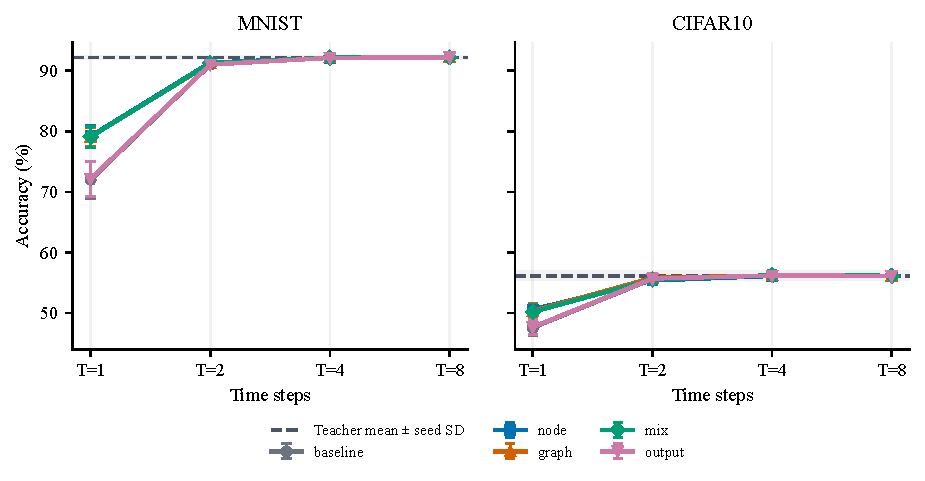
\includegraphics[width=\textwidth]{../figures/accuracy_curves.pdf}\caption{Full validation fidelity across three teacher seeds. Error bars are sample SD. Teacher reference bands use the corresponding validation mean and SD. All optimized conditions use the frozen smaller-step configuration.}\label{fig:accuracy}\end{figure*}

\begin{figure*}[t]\centering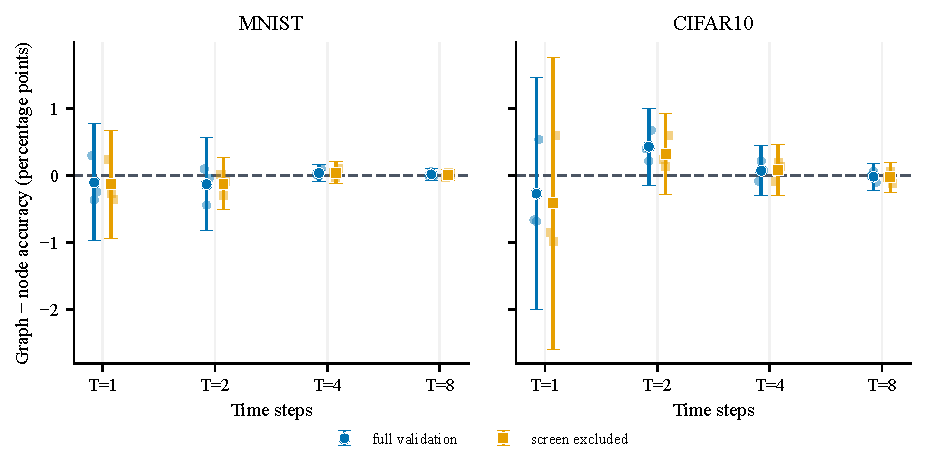
\includegraphics[width=\textwidth]{../figures/paired_objective.pdf}\caption{Graph-minus-local accuracy differences on full validation and the 4,488 examples outside the current screen. Small markers show each teacher seed; intervals use the paired three-seed $t$ distribution with two degrees of freedom. Both subsets have historical exposure.}\label{fig:paired}\end{figure*}

\subsection{Error association and conditional location}

On the screen-excluded examples, graph-logit MSE is more correlated with flips than the four-node-site error aggregate in all twelve task/seed/low-prefix cells. Including the two MLP sites raises the local proxy correlation, while the output proxy remains stronger on average. Teacher margin is more predictive still: mean flip-ranking AUC for negative margin is 0.77/0.96 on MNIST $T=1/2$ and 0.73/0.90 on CIFAR10, compared with 0.67/0.61 and 0.59/0.59 for graph-logit MSE. These are marginal associations on the same graphs.

The ideal interventions identify a different question: which quantizers conditionally cause the observed discrepancy? At $T=1$, restoring all four node sites closes 80.4\%/45.2\% of the MNIST/CIFAR10 disagreement gaps, versus 8.8\%/14.9\% when restoring only the two readout sites.

The first node site alone closes about 54.1\%/23.5\%, and gives the largest individual-site accuracy recovery in both tasks. This supports an important upstream quantization effect in this architecture rather than a dominant readout-only explanation. At $T=2$, node and readout group effects are closer on CIFAR10. Restoring all sites reproduces the folded teacher exactly in these runs. These continuous-valued interventions restore different numbers of sites and can interact; their effects are conditional rather than additive.

\begin{table*}[t]\centering\footnotesize
\begin{tabular}{llrrrrr}\toprule
Task & $T$ & Baseline & First node (1) & All node (4) & Readout (2) & All sites (6) \\ \midrule
MNIST & 1 & 71.99 $\pm$ 3.04 & 84.88 $\pm$ 1.50 & 90.14 $\pm$ 0.25 & 74.17 $\pm$ 2.67 & 92.18 $\pm$ 0.20 \\
MNIST & 2 & 91.00 $\pm$ 0.29 & 91.71 $\pm$ 0.23 & 91.95 $\pm$ 0.21 & 91.49 $\pm$ 0.44 & 92.18 $\pm$ 0.20 \\
CIFAR10 & 1 & 47.59 $\pm$ 1.26 & 51.12 $\pm$ 1.14 & 52.97 $\pm$ 0.33 & 50.19 $\pm$ 1.25 & 56.15 $\pm$ 0.69 \\
CIFAR10 & 2 & 55.63 $\pm$ 0.87 & 55.78 $\pm$ 0.90 & 55.95 $\pm$ 0.75 & 55.87 $\pm$ 0.74 & 56.15 $\pm$ 0.69 \\
\bottomrule\end{tabular}
\caption{Ideal-site validation accuracy (percent), mean $\pm$ sample SD over three teachers. Parentheses give numbers of restored nonlinearities. These are continuous-valued diagnostic interventions with zero fitted offsets, not deployable spiking competitors or budget-matched algorithms. All six ideal sites recover the teacher.}\label{tab:ideal}\end{table*}


\subsection{Calibration and software cost}

Local and graph conditions share their inference computation and differ only in fitted initial states. Their measured times are nearly coincident (Figure~\ref{fig:latency}). The one-tick baseline core averages 0.366/0.493 ms per graph on MNIST/CIFAR10, versus 0.152/0.157 for the teachers.

The conversion core at $T=8$ averages 2.407/3.451 ms per graph. These are means of three per-seed batch medians divided by 32, with raw repeated timings retained. The diagnostic core returns site activations as well as logits, so these ratios describe its actual implementation rather than a best-achievable backend bound.

The three-seed mean times of the 64-update local/graph calibration loops are about 1.1--2.6 seconds per low-prefix condition, excluding shared data loading, checks and target preparation. Dense graph projections and edge reductions run at every tick regardless of zero-event counts. The arithmetic ledger records those projections and reductions as a partial lower bound; it excludes neuron-state arithmetic and memory traffic and therefore cannot serve as a complete energy estimate. Physical energy remains unmeasured.

\begin{figure*}[p]\centering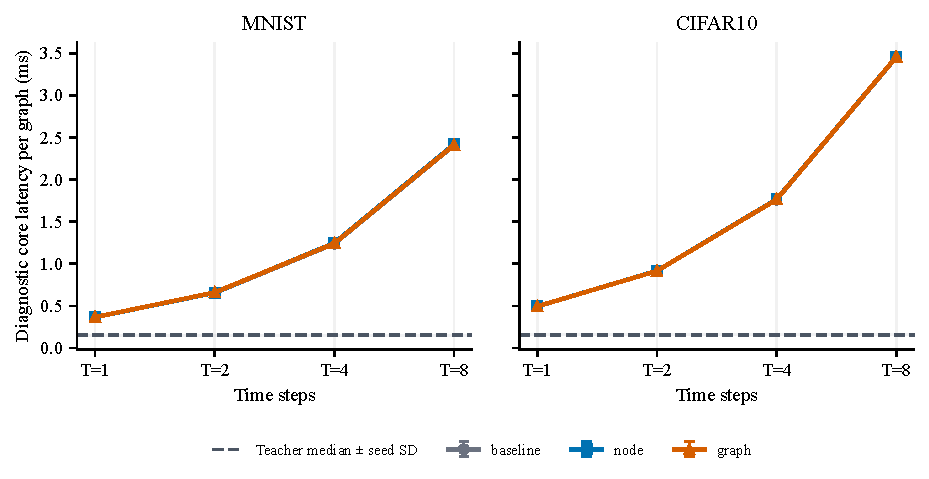
\includegraphics[width=\textwidth]{../figures/latency.pdf}\caption{Synchronized diagnostic-core runtime on a fixed cached batch of 32 graphs. Points summarize three teacher-seed medians; error bars show their sample SD. Each condition has ten warmups and thirty randomized interleaved repeats. Data transfer is excluded.}\label{fig:latency}\end{figure*}

\subsection{Failure conditions}

The initial $10^{-2}$ step size increased MNIST $T=2$ hard training logit MSE from 0.685 to 0.966; the single smaller-step correction improved optimization but did not produce a stable graph-objective advantage. Shuffling targets substantially degrades fidelity at every tested prefix, establishing target-correspondence sensitivity. That result is compatible with ordinary distillation and does not identify a topology-specific mechanism. The unchanged original screen, all per-seed endpoints and individual-site interventions accompany the summaries.

\begin{table*}[p]\centering\footnotesize
\begin{tabular}{llrrrrrrrr}\toprule
Task & Seed & $T$ & ANN & Uncalibrated & Local & Graph & Mixed & Output & Shuffled \\ \midrule
MNIST & 41 & 1 & 90.94 & 74.46 & 78.48 & 78.68 & 78.88 & 74.62 & 39.10 \\
MNIST & 41 & 2 & 90.94 & 90.16 & 89.96 & 90.13 & 90.26 & 90.10 & 53.74 \\
MNIST & 41 & 4 & 90.94 & 90.94 & 90.86 & 90.79 & 90.97 & 90.94 & 52.57 \\
MNIST & 41 & 8 & 90.94 & 90.93 & 90.95 & 90.93 & 90.93 & 90.93 & 72.82 \\
\addlinespace[2pt]
MNIST & 42 & 1 & 91.32 & 70.92 & 80.61 & 80.90 & 81.06 & 71.14 & 41.47 \\
MNIST & 42 & 2 & 91.32 & 90.64 & 90.38 & 90.65 & 90.59 & 90.71 & 57.87 \\
MNIST & 42 & 4 & 91.32 & 91.33 & 91.33 & 91.33 & 91.27 & 91.34 & 69.98 \\
MNIST & 42 & 8 & 91.32 & 91.30 & 91.30 & 91.34 & 91.36 & 91.30 & 74.52 \\
\addlinespace[2pt]
MNIST & 43 & 1 & 90.81 & 68.93 & 76.41 & 76.53 & 76.90 & 69.07 & 38.85 \\
MNIST & 43 & 2 & 90.81 & 89.67 & 89.90 & 89.99 & 89.72 & 89.70 & 45.05 \\
MNIST & 43 & 4 & 90.81 & 90.85 & 90.82 & 90.91 & 90.80 & 90.86 & 59.14 \\
MNIST & 43 & 8 & 90.81 & 90.81 & 90.82 & 90.82 & 90.80 & 90.81 & 69.85 \\
\addlinespace[2pt]
CIFAR10 & 41 & 1 & 54.87 & 45.48 & 49.87 & 49.13 & 49.46 & 45.75 & 22.84 \\
CIFAR10 & 41 & 2 & 54.87 & 53.87 & 54.27 & 54.13 & 54.17 & 53.88 & 28.09 \\
CIFAR10 & 41 & 4 & 54.87 & 54.88 & 54.86 & 54.92 & 54.85 & 54.89 & 38.92 \\
CIFAR10 & 41 & 8 & 54.87 & 54.93 & 54.88 & 54.86 & 54.92 & 54.93 & 48.74 \\
\addlinespace[2pt]
CIFAR10 & 42 & 1 & 54.94 & 47.90 & 49.82 & 50.48 & 50.08 & 48.10 & 22.89 \\
CIFAR10 & 42 & 2 & 54.94 & 54.00 & 54.01 & 54.33 & 54.67 & 53.97 & 28.89 \\
CIFAR10 & 42 & 4 & 54.94 & 54.86 & 54.99 & 54.96 & 54.95 & 54.87 & 38.54 \\
CIFAR10 & 42 & 8 & 54.94 & 54.95 & 54.93 & 54.97 & 54.97 & 54.95 & 48.05 \\
\addlinespace[2pt]
CIFAR10 & 43 & 1 & 55.01 & 47.01 & 50.08 & 49.63 & 49.62 & 47.14 & 27.29 \\
CIFAR10 & 43 & 2 & 55.01 & 54.34 & 54.25 & 54.65 & 54.43 & 54.40 & 28.37 \\
CIFAR10 & 43 & 4 & 55.01 & 54.98 & 55.03 & 55.02 & 54.91 & 54.98 & 32.81 \\
CIFAR10 & 43 & 8 & 55.01 & 55.00 & 55.04 & 55.08 & 55.08 & 54.99 & 42.16 \\
\addlinespace[2pt]
\bottomrule\end{tabular}
\caption{Individual frozen test accuracies (percent) underlying Table~\ref{tab:test}. Each row uses the same teacher checkpoint and all 10,000 official test graphs, with no fitting at test time. The official test split has historical exposure.}\label{tab:individual}\end{table*}



\section{Discussion}
Objective choice changes what the calibration procedure is encouraged to preserve, but the hard event dynamics, surrogate derivative and optimization budget mediate that choice. A graph-logit loss can improve a decision without minimizing every local error, and lower reconstruction error can coexist with a classification loss when samples cross different margins. The matched results should therefore be interpreted jointly through accuracy, agreement and reconstruction error rather than a single objective value.

Numerical determinism is especially relevant at event thresholds. In an early real-data CUDA equivalence check, source/core output discrepancies changed between repeated evaluations. Deterministic execution restored bitwise equality at all checked prefixes. This observation is consistent with small aggregation-order perturbations crossing discrete thresholds. It motivates controlling numerical execution before attributing differences to a calibration mechanism.

Fidelity and runtime describe different properties. The current dense graph projections and edge reductions execute even when many events are zero. Signed event selection, membrane updates and time-prefix iteration add work. A lower event count alone consequently gives neither a measured GPU speedup nor a hardware energy result.

\section{Limitations}
The controlled method comparison covers two superpixel tasks with one fixed GCN family and three teacher training seeds. Historically exposed validation/test endpoints and a post-screen learning-rate correction limit confirmatory inference. The surrogate optimizer evaluates one bounded implementation of potential calibration, not all possible graph-aware objectives or optimizers. The output-bias control has a smaller parameter budget. Target shuffling tests correspondence rather than graph structure, and marginal error correlations do not establish a causal bottleneck. GatedGCN results provide contextual teacher/conversion endpoints, not evidence that the proposed calibration generalizes to dynamic gates. Runtime measurements cover a diagnostic PyTorch implementation and cached batches; the arithmetic ledger is partial and physical energy is unmeasured.

\section{Conclusion}
Local activation calibration captures substantial one-tick fidelity gains in the tested frozen GCN family. Direct graph-logit matching yields smaller changes that depend on task, seed and split. Better output-error correlation consequently does not suffice to establish a better calibration objective. Ideal interventions identify an important early node-quantization effect, while dense software execution remains costly even at short prefixes. The evidence supports a bounded empirical study and motivates stronger source-faithful controls, structure-preserving mechanism tests and broader confirmation.


\bibliographystyle{plainnat}
\bibliography{references}
\end{document}
